%%
%% Copyright 2007, 2008, 2009 Elsevier Ltd
%%
%% This file is part of the 'Elsarticle Bundle'.
%% ---------------------------------------------
%%
%% It may be distributed under the conditions of the LaTeX Project Public
%% License, either version 1.2 of this license or (at your option) any
%% later version.  The latest version of this license is in
%%    http://www.latex-project.org/lppl.txt
%% and version 1.2 or later is part of all distributions of LaTeX
%% version 1999/12/01 or later.
%%
%% The list of all files belonging to the 'Elsarticle Bundle' is
%% given in the file `manifest.txt'.
%%

%% Template article for Elsevier's document class `elsarticle'
%% with harvard style bibliographic references
%% SP 2008/03/01
%%
%%
%%
%% $Id: elsarticle-template-harv.tex 4 2009-10-24 08:22:58Z rishi $
%%
%%

%%% Document Class 
%--------------------------------------------------------------------------------- 

\documentclass[review,3p]{elsarticle}
%\documentclass[final,5p,10pt,twocolumn]{elsarticle}
% Use the option review to obtain double line spacing
%% \documentclass[authoryear,preprint,review,12pt]{elsarticle}

%% Use the options 1p,twocolumn; 3p; 3p,twocolumn; 5p; or 5p,twocolumn
%% for a journal layout:
%% \documentclass[final,authoryear,1p,times]{elsarticle}
%% \documentclass[final,authoryear,1p,times,twocolumn]{elsarticle}
%% \documentclass[final,authoryear,3p,times]{elsarticle}
%% \documentclass[final,authoryear,3p,times,twocolumn]{elsarticle}
%% \documentclass[final,authoryear,5p,times]{elsarticle}
%% \documentclass[final,authoryear,5p,times,twocolumn]{elsarticle}



%%% Packages 
%--------------------------------------------------------------------------------- 

%% if you use PostScript figures in your article
%% use the graphics package for simple commands
% \usepackage{graphics}
%% or use the graphicx package for more complicated commands

%% or use the epsfig package if you prefer to use the old commands
%% \usepackage{epsfig}

%% The amssymb package provides various useful mathematical symbols
% \usepackage{amssymb}
%% The amsthm package provides extended theorem environments
% \usepackage{amsthm}

%% The fleqn package allows left aligned equations
\usepackage{graphicx}
%\usepackage{lineno}
\usepackage{fleqn}
\usepackage{tikz}
\usepackage{pgfplots}
\usepackage{booktabs}
\usepackage{multirow}
\usepackage{amsmath}
\usepackage{nomencl}
\usepackage{framed} % Framing content
\usepackage{multicol} % Multiple columns environment
\usepackage[nodots]{numcompress}
\usetikzlibrary{pgfplots.groupplots}
%\usepackage{ifthen}

%\usepackage{hyperref}

%\hypersetup{ 
%    colorlinks,% 
%    citecolor=black,% 
%    filecolor=black,% 
%    linkcolor=black,% 
%    urlcolor=black 
%} 


\setlength{\nomitemsep}{-\parskip} % Baseline skip between items

\renewcommand*\nompreamble{\begin{multicols}{2}}
\renewcommand*\nompostamble{\end{multicols}}

%\renewcommand{\nomname}{Abkürzungsverzeichnis}  
%\renewcommand{\nomgroup}[B]{subscript} 

\RequirePackage{ifthen}
\renewcommand{\nomgroup}[1]{%
\ifthenelse{\equal{#1}{G}}{\item[\textbf{Greek Symbols}]}{
\ifthenelse{\equal{#1}{S}}{\item[\textbf{Subscripts}]}{}}
\ifthenelse{\equal{#1}{A}}{\item[\textbf{Acronyms}]}{
\ifthenelse{\equal{#1}{M}}{\item[\textbf{Symbols}]}{}}

}

%uncomment this when 'preprint submitted to' is to be removed
%\makeatletter
%\def\ps@pprintTitle{%
%  \let\@oddhead\@empty
%  \let\@evenhead\@empty
%  \def\@oddfoot{\reset@font\hfil\thepage\hfil}
%  \let\@evenfoot\@oddfoot
%}
%\makeatother

\makeindex
\makenomenclature

%% The lineno packages adds line numbers. Start line numbering with
%% \begin{linenumbers}, end it with \end{linenumbers}. Or switch it on
%% for the whole article with \linenumbers after \end{frontmatter}.
%% \usepackage{lineno}

%% natbib.sty is loaded by default. However, natbib options can be
%% provided with \biboptions{...} command. Following options are
%% valid:

%%   round  -  round parentheses are used (default)
%%   square -  square brackets are used   [option]
%%   curly  -  curly braces are used      {option}
%%   angle  -  angle brackets are used    <option>
%%   semicolon  -  multiple citations separated by semi-colon (default)
%%   colon  - same as semicolon, an earlier confusion
%%   comma  -  separated by comma
%%   authoryear - selects author-year citations (default)
%%   numbers-  selects numerical citations
%%   super  -  numerical citations as superscripts
%%   sort   -  sorts multiple citations according to order in ref. list
%%   sort&compress   -  like sort, but also compresses numerical citations
%%   compress - compresses without sorting
%%   longnamesfirst  -  makes first citation full author list
%%
%\biboptions{sort&compress}
\biboptions{square,comma,sort&compress}

\journal{Energy}


%%% Main matter
%--------------------------------------------------------------------------------- 

\begin{document}

\begin{frontmatter}

%% Title, authors and addresses

%% use the tnoteref command within \title for footnotes;
%% use the tnotetext command for the associated footnote;
%% use the fnref command within \author or \address for footnotes;
%% use the fntext command for the associated footnote;
%% use the corref command within \author for corresponding author footnotes;
%% use the cortext command for the associated footnote;
%% use the ead command for the email address,
%% and the form \ead[url] for the home page:
%%
%% \title{Title\tnoteref{label1}}
%% \tnotetext[label1]{}
%% \author{Name\corref{cor1}\fnref{label2}}
%% \ead{email address}
%% \ead[url]{home page}
%% \fntext[label2]{}
%% \cortext[cor1]{}
%% \address{Address\fnref{label3}}
%% \fntext[label3]{}

\title{System analysis and optimisation of a Kalina Split-cycle for waste heat recovery on large marine diesel engines}

%% use optional labels to link authors explicitly to addresses:
%% \author[label1,label2]{<author name>}
%% \address[label1]{<address>}
%% \address[label2]{<address>}

\author{Ulrik Larsen\corref{cor}}\cortext[cor]{Principal corresponding author. Tel.: +4553250303} \ead{ular@mek.dtu.dk}
\author{Tuong-Van Nguyen\corref{}}
\author{Thomas Knudsen\corref{}}
\author{Fredrik Haglind\corref{}} 

\address{Section of Thermal Energy, Department of Mechanical Engineering, Technical University of Denmark,\\ Building 403, Nils Koppels All\'{e}, 2800 Kongens Lyngby, Denmark}

\begin{abstract}
%% Text of abstract
Waste heat recovery systems can produce power from heat without using fuel or emitting CO$_2$, therefore their implementation is  becoming increasingly relevant. The Kalina cycle is proposed as an efficient process for this purpose. The main reason for its high efficiency is the non-isothermal phase change characteristics of the ammonia-water working fluid. 
The present study investigates a unique type of Kalina process called the Split-cycle, applied to the exhaust heat recovery from large marine engines. In the Split-cycle, the working fluid concentration can be changed during the evaporation process in order to further improve the match between the heat source and working fluid temperatures.
We present a system analysis to identify the governing mechanisms of the process, including a comparison of the efficiency of the Split-cycle and a conventional Kalina cycle and an investigation of the effects of using reheat in both cases. 
Results of a multi-variable optimisation effort using a genetic algorithm suggest that the Split-cycle process can obtain a thermal efficiency of 23.2\% when using reheat compared to 20.8\% for a conventional reference Kalina cycle. Reheat is advantageous for both the reference cycle and the Split-cycle process and can increase the thermal efficiency by 3.4\% and 5.9\%, respectively.







\end{abstract}

\begin{keyword} %% keywords here, in the form: keyword \sep keyword
Kalina Split-cycle \sep Process integration \sep Waste heat recovery \sep Reheat



\end{keyword}

\end{frontmatter}

%\linenumbers
%% main text




\section{Introduction}
\label{sec:introduction}
Waste heat recovery (WHR) systems are able to generate mechanical power and electricity without any fuel input and associated CO$_2$ emissions. Hence, with rising fuel prices and increased environmental awareness, motivation is growing for integrating these systems to improve the energy efficiency of various processes. An example is a WHR system for large marine engines in the present study.

Organic Rankine cycles (ORC) and Kalina cycles are among the most frequently proposed alternatives to steam Rankine cycle WHR systems. At the scale of application studied in the present work, i.e. a net power output of 1-5 MW, both power cycles may be viable \cite{Tchanche20113963,Jonsson2001c}. Bombarda et al. \cite{Bombarda2010b} compared the two processes for a heat source temperature level of 346$^\circ$C and found that both cycles, when optimised, produced almost equal net power outputs. While the present study does not directly compare the ORC with the Kalina cycle, this work is based on the boundary conditions used in the work of Bombarda et al. \cite{Bombarda2010b}, in order to make comparisons about the power cycle performance for the same application.

\begin{table*}[htbp]
  \begin{framed}
  \small
    \printnomenclature
  \end{framed}
\end{table*}

The main reason for the relatively high thermal efficiency of the Kalina cycle is the non-isothermal evaporation and condensation processes which occur because the working fluid is a zeotropic mixture of two fluids \cite{Wang2009a}. This enables a close matching of the temperatures of the heat source and the working fluid in the boiler, and between the heat sink and working fluid in the condenser(s). Among the many variations of the cycle, Alexander Kalina, the inventor of the Kalina cycle, has proposed a unique type of cycle layout that enables an even better match between the temperatures of the heat source and the working fluid. This is achieved by having an additional system of mixers and splitters to form two streams of working fluid with different mixture compositions that enter the boiler separately. A full description of this configuration, which Kalina  named the Split-cycle (SC) \cite{Kalina1986a}, is provided in section \ref{sec:split_cycle}.

In the literature \cite{Kalina1985a,Kalina1986a}, the conceptual idea of the SC is described, but no thermodynamic analyses or modelling efforts are presented. Previous work by the present authors \cite{larsen2012} investigated a method for the optimisation of this special Kalina process, finding that compared to a conventional Kalina cycle the SC process may be able to improve the thermal efficiency from 20.1\% to 21.5\%. However, the optimisation methodology was limited to including only the boiler and turbine components. 

Further analyses showed that the potential of the process could not be found using this methodology, but an optimisation of the entire process is required. Due to the complexity of the process, a relatively large number of parameters needs to be optimised simultaneously. Thus using a comprehensive multi-variable optimisation method is required.

This study presents, first, a system analysis with the objective of identifying the governing mechanisms of the process. Second, the potential of the Split-cycle process, in terms of conversion efficiency, is investigated in the context of the marine diesel engine WHR using a genetic algorithm optimisation methodology. The performance of a reference Kalina process is compared to the Split-cycle process, and the potential effect of implementing reheat in both cycles is studied.

Section \ref{sec:processDescriptions} presents descriptions of the modelled processes, while section \ref{sec:methodology} presents the modelling methodology and the optimisation algorithm. An analysis of the most important process mechanisms influencing the overall process efficiency is presented in section \ref{sec:resultsAnalysis} along with the optimisation results. Section \ref{sec:discussion} provides a brief discussion of the findings.


\nomenclature[A]{WHR}{Waste heat recovery}
\nomenclature[A]{ORC}{Organic Rankine cycle}
\nomenclature[A]{SC}{Split-cycle}
\nomenclature[A]{SUP}{Superheated state}
\nomenclature[A]{SUB}{Subcooled state}

\nomenclature[M]{$\dot{m}$}{Mass flow rate (kg/s)}
\nomenclature[M]{$h$}{Specific enthalpy (kJ/kg)}
\nomenclature[M]{$x$}{Concentration by mass (-)}
\nomenclature[M]{$P$}{Pressure (bar)}
\nomenclature[M]{$q$}{Vapour quality (-)}







\section{Process descriptions}
\label{sec:processDescriptions}
The reference Kalina process layout and the process conditions used throughout were the same as those presented in the work of Bombarda et al. \cite{Bombarda2010b}. Both the reference cycle and the Split-cycle were evaluated with and without using reheat in the turbine, in order to determine the influence of this technique on the processes. 

In the following, the solution concentration running through the turbine is referred to as the \emph{working solution}, and the terms \emph{lean} and \emph{rich} refer to a low and a high concentration of ammonia in the solution, respectively.

\subsection{Reference Kalina cycle}
\label{sec:kalina_cycle}
\begin{figure*}[htbp]
\centering
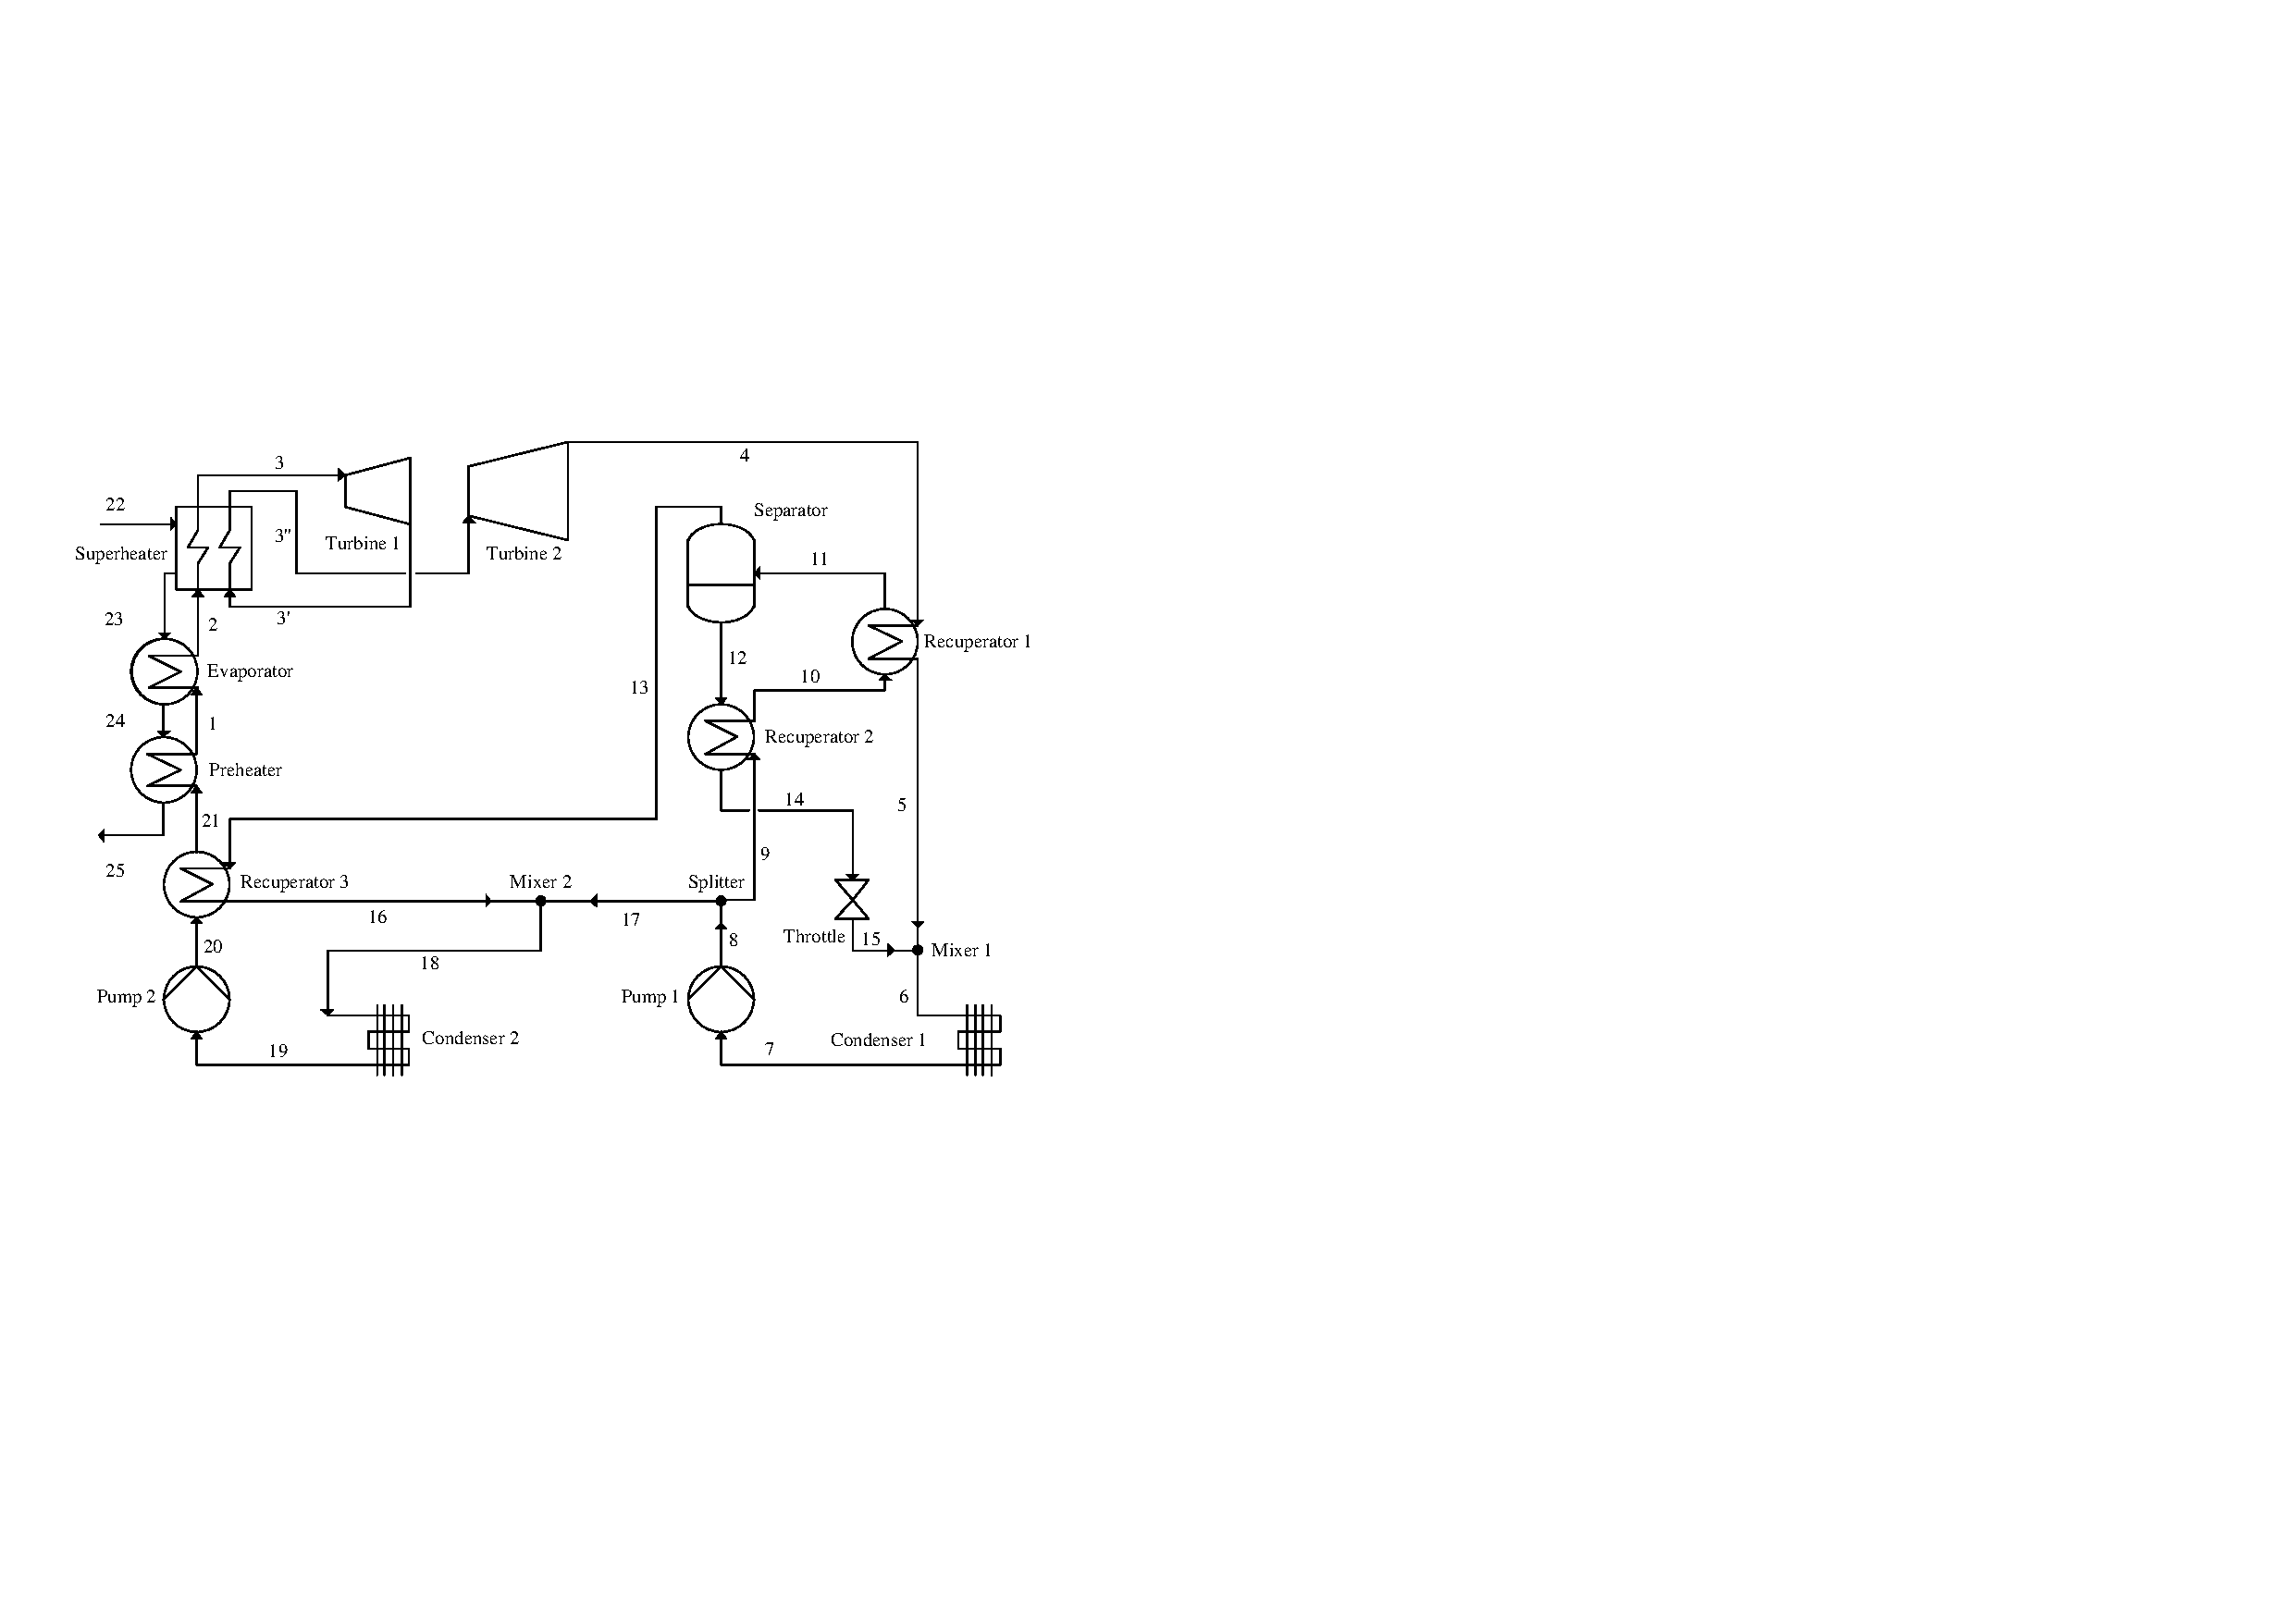
\includegraphics[width=0.9\linewidth]{figures/Drawing_Kalina_Baselinevsd.pdf}
\caption{Sketch of the Kalina reference process with reheat}
\label{fig:kalina_cycle}
\end{figure*}

Figure \ref{fig:kalina_cycle} illustrates the flow diagram of the reference Kalina process with reheat. Starting from (21) to (1), the preheated working fluid is evaporated and superheated in the boiler before it enters the turbine (3). In the process layout that includes the reheat technique, the outlet stream from the turbine (3') is heated in the boiler before entering (3'') a second turbine. When reheat is not included in the process, stream (3) runs directly from the turbine outlet (4) to Recuperator 1. From the stream (4) heat is transferred to the stream (10) in Recuperator 1. The stream (5) is then mixed with an ammonia lean stream from the separator (15) to form a leaner solution. This solution is condensed (7) and after being pumped to an intermediate pressure level, the stream (8) is divided into two streams (9) and (17). The stream (9) is heated in Recuperator 2 and in Recuperator 1 to a partially evaporated state. It then enters the separator which separates the stream into a lean liquid (12) and a very rich vapour (13). Heat from stream (13) is used to preheat stream (20) in Recuperator 3, and the stream (16) is then mixed with a leaner solution (17) to form the working solution (18). This stream is finally condensed and pumped to the boiler pressure. 





\subsection{Kalina Split-cycle}
\label{sec:split_cycle}
\begin{figure*}[htbp]
\centering
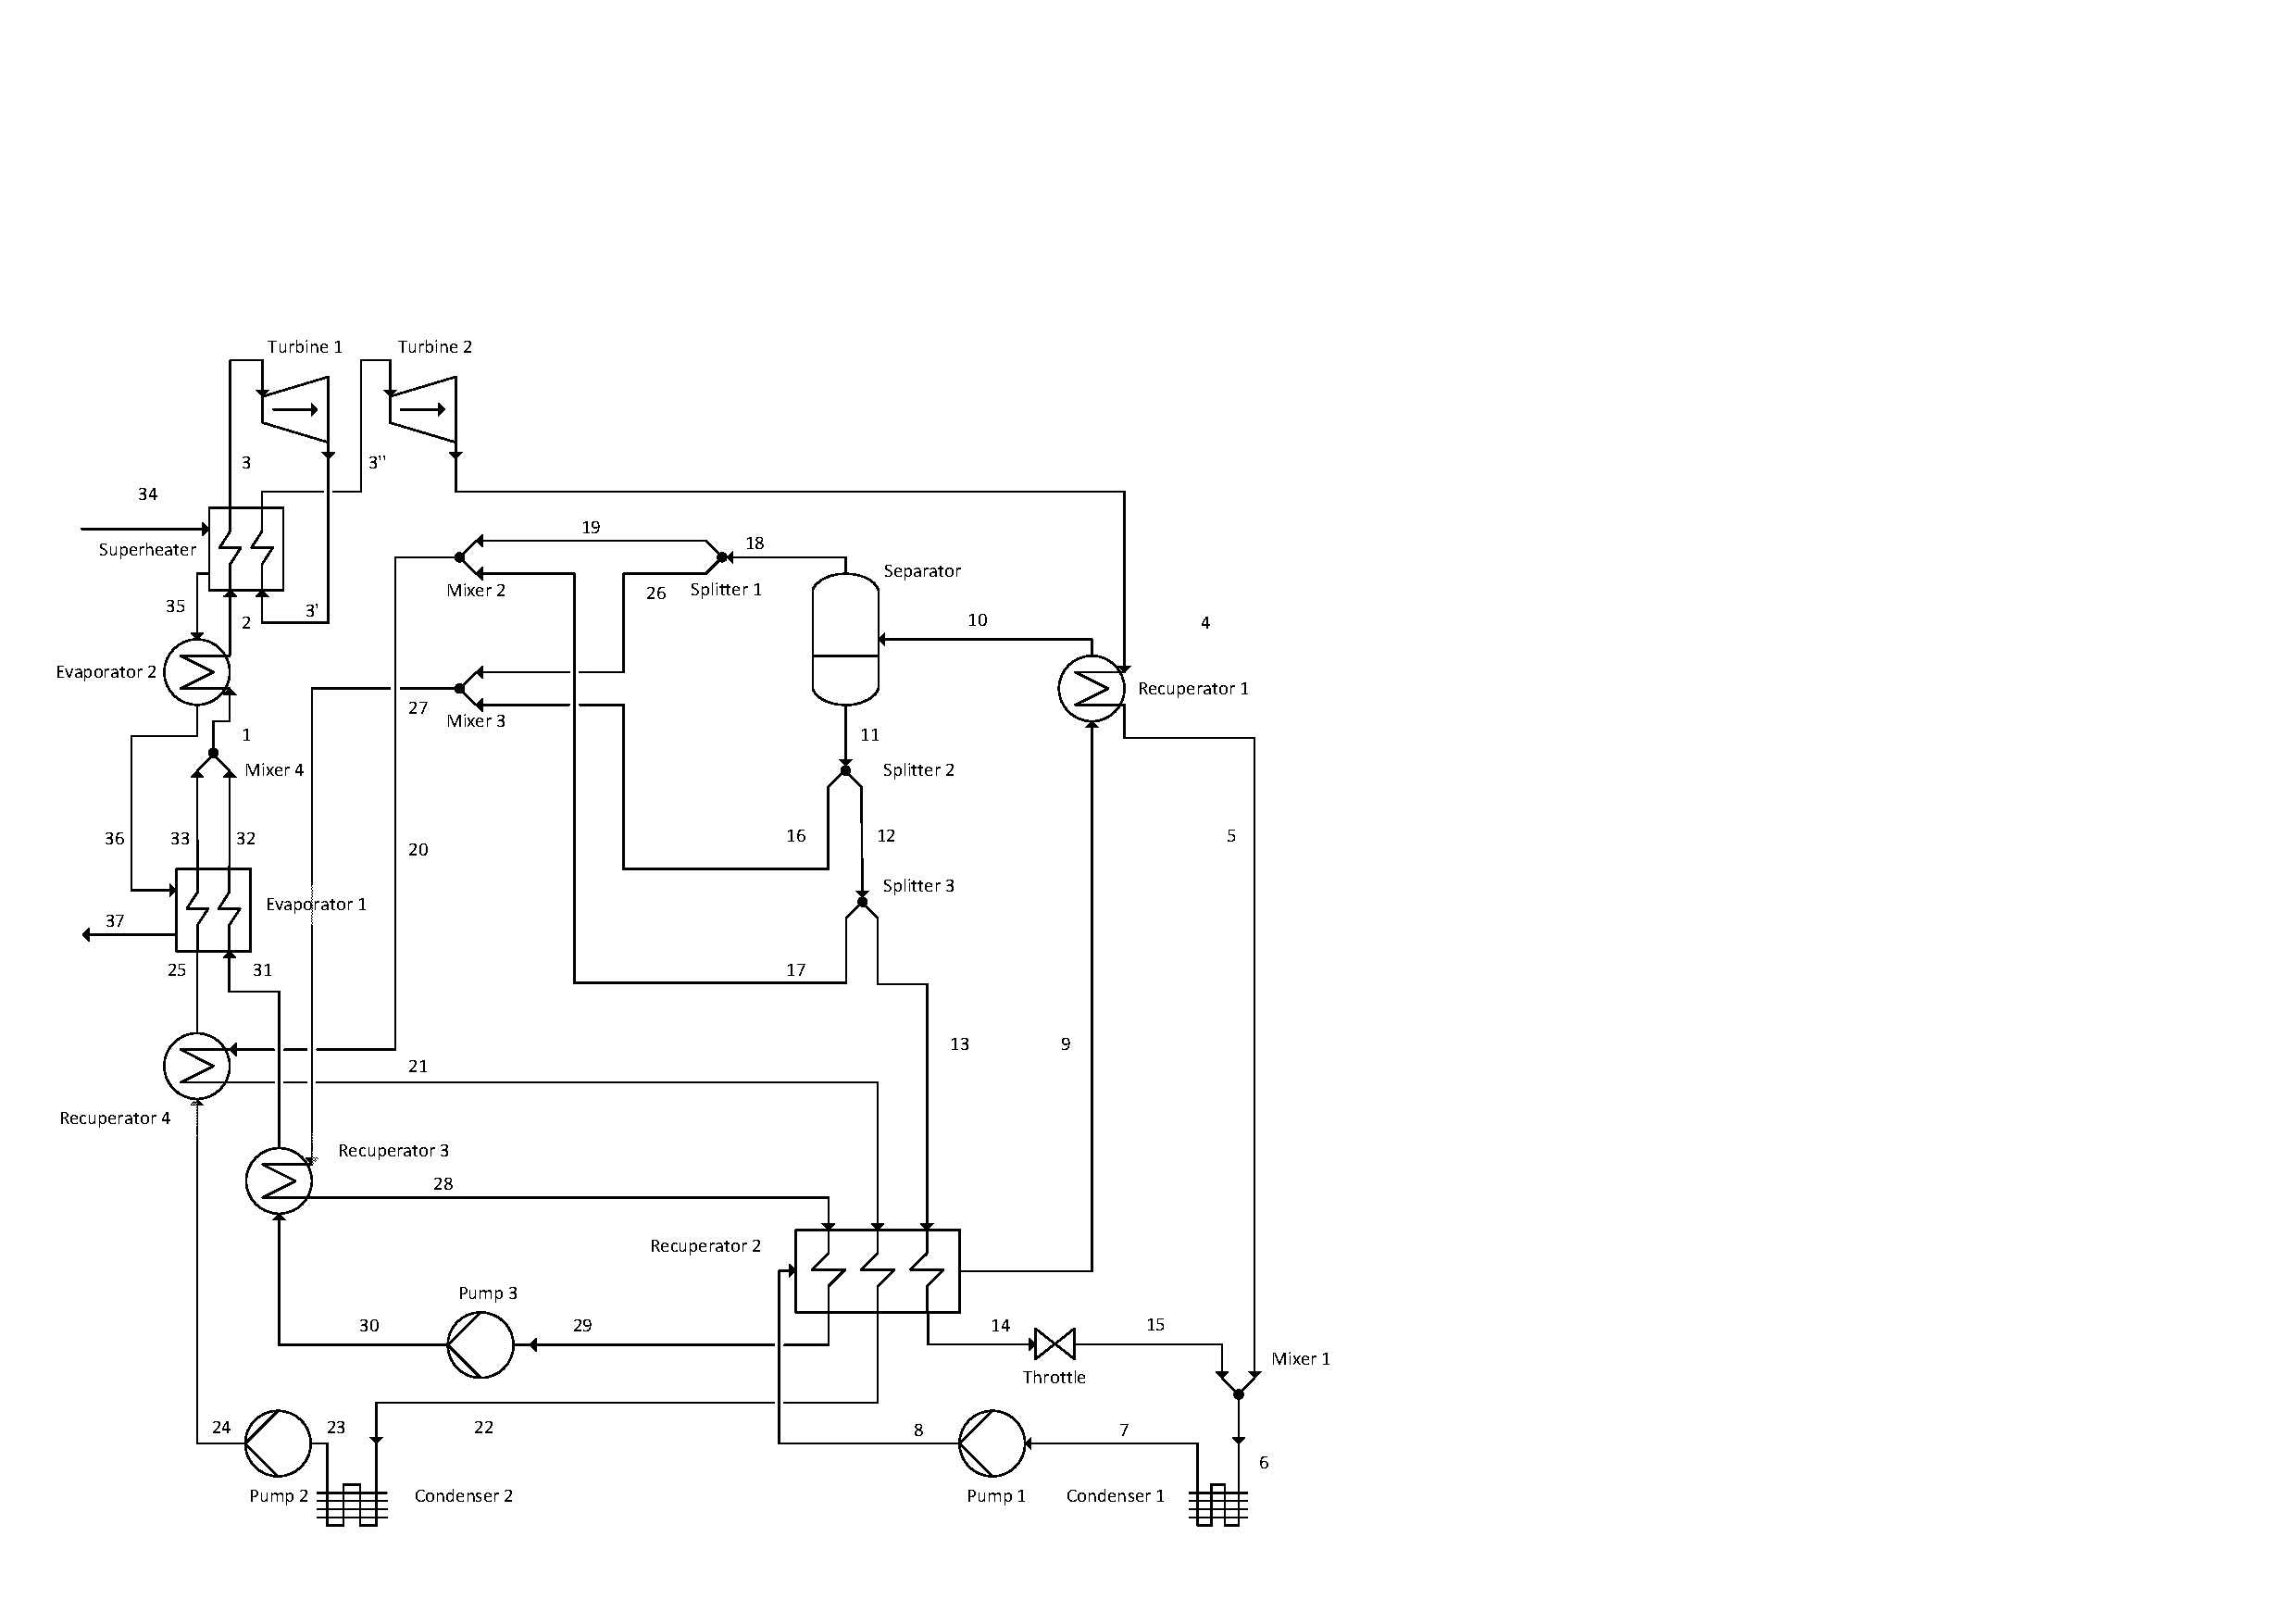
\includegraphics[width=1.0\linewidth]{figures/Drawing_Kalina_Split.pdf}
\caption{Sketch of the Kalina Split-cycle process}
\label{fig:split_cycle}
\end{figure*}

Figure \ref{fig:split_cycle} illustrates the flow diagram of the Split-cycle process. To maintain focus on the special split stream boiler, the Split-cycle configuration modelled in this work was designed to have a minimum number of components needed for evaluating the concept. Hence, the SC presented here is based on the same principles as the reference Kalina cycle, with some important differences. 

Two streams of different ammonia concentration enter the boiler, a rich stream (25) and a lean stream (31). Before being mixed (Mixer 4), the rich stream is fully evaporated, and the lean stream is heated to the bubble point state. The aim of this arrangement is to lower the temperatures in the overall process going from liquid (25,31) to vapour (2). To be able to produce these two streams with the desired concentrations and mass flow rates, an additional mixing subsystem, consisting of three splitters and two mixers, is also needed. 

The gradient of the evaporation temperature curve can to some degree be adjusted to the temperature profile of the heat source by selecting the optimal composition of each of the two streams, as illustrated in Fig. \ref{fig:theory}. The line from (25,31) to the point ($T_{r,b}$)\nomenclature[S]{r}{Rich ammonia concentration} \nomenclature[S]{b}{Bubble point}represents the preheat stage. From here to points (1), (2) and (3) the fully drawn line represents the heat transfer when using the Split-cycle configuration. The upper dashed line represents how the heat transfer would be if the two streams were combined into a single stream. The point ($T_{b}$) signifies the bubble point of the combined stream, and it is clear that the temperature difference at the pinch point is much smaller and possibly violated in this case. The lower dashed line from ($T_{r,b}$) through (2a) to (2), shows how the heat transfer would occur if only the rich stream concentration was used. Evaporation would take place at lower temperatures possibly leading to a lower thermal efficiency. 



\begin{figure*}[htpb]
\centering
\begin{tikzpicture}[scale=0.9]

\begin{axis}[xlabel={Accumulated heat transfer},
	ylabel={Temperature},
	axis lines*=left,
	legend pos=outer north east,
	no markers,
	xticklabels={,,},
	yticklabels={,,}
	]

\addplot [style=thick] table[x index=0,y index=1,col sep=space] {theory.data}; %split
\addplot table[x index=0,y index=1,col sep=space] {theoryHeatSource.data}; %heat source
\addplot [style=dashed] table[x index=0,y index=1,col sep=space] {theoryRich.data}; %rich alone
\addplot [style=dashed] table[x index=0,y index=1,col sep=space] {theoryComp.data}; %composite

\node[] at (40,1) {$25,31$}; 
\node[] at (100,22) {$T_{r,b}$};
\node[] at (50,50) {$T_{b}$};
\node[] at (200,60) {$1$};
\node[] at (300,70) {$2$};
\node[] at (270,45) {$2a$};
\node[] at (400,92) {$3$};
\node[] at (0,25) {$37$};
\node[] at (400,112) {$34$};

\end{axis}
\end{tikzpicture}

\caption{Sketch of T-Q diagram of the heat recovery system to explain the Split-cycle}
\label{fig:theory}
\end{figure*}






Kalina argued \cite{Kalina1986a} that the state of the rich stream at point (33) (Fig. \ref{fig:split_cycle}) should ideally be at the dew point and that the lean stream at point (32) should be at the bubble point, before the mixing of the two streams. The two streams should also have similar temperatures and pressures in order to minimise the entropy generation in this section of the boiler. We decided to adopt these constraints without further analysis to focus on the full process analysis. However, an entropy generation analysis is planned for future work to verify this claim. In the following, these conditions are referred to as the SC boiler constraints. 

A direct consequence of the SC boiler constraints is that, once the ammonia concentration of one of the streams, (25) or (31), has been chosen, the concentration of the other is fixed in order to satisfy the equilibrium conditions. Additionally, when the boiler pressure and the concentration in one stream are chosen, the temperature of the working fluid streams out of evaporator 1 is fixed. Both are illustrated in the example shown in Fig. \ref{fig:bubbleDew}. As shown, the mixing temperature decreases and the lean stream concentration increases, as the rich stream concentration increases. 



\begin{figure}[htpb]
\centering
\begin{tikzpicture}[scale=0.9]

\begin{axis}[xlabel={Rich stream ammonia concentration},
	%xmin=0.75, xmax=1.0,
	ymin=0.2,
	axis x line*=bottom,
	axis y line*=left,
	ylabel={Lean stream ammonia concentration},
	ylabel near ticks,
	legend style={legend pos=south west,font=\small, draw=none} ,
	]

\addplot [mark=triangle*, mark options={fill=black}] table[x index=0,y index=1,col sep=space] {data/bubbleDewPoints.txt};
\addlegendentry{Concentration}

\end{axis}

\begin{axis}[xlabel={},
	%xmin=0.75, xmax=1.0,
	ymin=100,
	axis x line*=bottom,
	hide x axis,
	axis y line*=right,
	ylabel={Mixing temperature ($^\circ$C)},
	ylabel near ticks,
	legend style={legend pos=south east,font=\small, draw=none} ,
	]

\addplot table[x index=0,y index=2,col sep=space] {data/bubbleDewPoints.txt};
\addlegendentry{Temperature}

\end{axis}
\end{tikzpicture}

\caption{Equilibrium conditions for Evaporator 1 outlet}
\label{fig:bubbleDew}
\end{figure}







%--------------------------------------------------------------------------
\section{Methodology}
\label{sec:methodology}
This section describes the models and conditions used as well as the optimisation methodology. In previous work \cite{larsen2012} the authors derived a preliminary optimisation methodology for the Split-cycle process. Subsequent work demonstrated that a need for a more comprehensive approach exists, mainly because of the strong influence of the turbine exhaust pressure on the process net power output; therefore the previous methodology and models were further developed to include the entire Split-cycle process. 


\subsection{General modelling conditions}
Table \ref{tab:modelingConditions} presents the process parameters common for all simulations. The heat source data was adopted from Bombarda et al. \cite{Bombarda2010b} being an exhaust gas stream from two marine diesel engines, with the following molar composition 74.6\% N$_2$, 11.7\% O$_2$, 6.7\% H$_2$O, 5.9\% CO$_2$ and 1.1\% Ar and a total mass flow rate of 35 kg/s. 

Pressure and heat losses were neglected in the models, to investigate the full potential of the cycles. All flows were considered homogeneous in terms of temperature, pressure and solution concentration, and the models were developed for steady-state conditions.


\begin{table}
\centering
\caption{Process parameters and conditions}
%
\scriptsize
\begin{tabular}{lr}
\toprule
Heat source inlet temperature ($^\circ$C)  &        346 \\
Heat source outlet temperature ($^\circ$C)  &      127.7 \\
Turbine polytropic efficiency (\%) &          70.5 \\
Turbine mechanical efficiency (\%) &         96 \\
Pump isentropic efficiency (\%) &         70 \\
Pump mechanical efficiency (\%) &         95 \\
$\Delta T_{PP}$ evaporators ($^\circ$C)  &       21.9 \\
Superheater approach ($^\circ$C) &         16 \\
$\Delta T_{PP}$ recuperators ($^\circ$C)&        5.0 \\
Cooling water inlet temperature ($^\circ$C) &         25 \\
$\Delta T_{PP}$ condenser ($^\circ$C) &         5.0 \\


\bottomrule
\end{tabular}  
\label{tab:modelingConditions}
\end{table}


It was assumed for the optimisation cases that the feasible upper limit for the high pressure of the processes is 130 bar to avoid supercritical pressures and possibly excessive costs.


\subsection{Subsystem models}
\label{sec:subsystemModels}
The preliminary optimisation methodology was based on the SC boiler constraints. Two subsystem models were made using MATLAB\textsuperscript{\textregistered} version 2010b  \cite{Mathworks2010} with thermodynamic properties obtained using NIST Refprop version 9 \cite{Lemmon2010}. The equation of state applied in Refprop for ammonia-water mixtures is a model derived by Tillner-Roth and Friend \cite{TillnerRoth1998} and is among the most accurate available \cite{Zhang20125309}. 

\subsubsection{Boiler and turbine model}
The boiler consists of two evaporators, a mixer and a superheater (with reheater). In order to find the minimum allowed temperature difference ($\Delta T_{PP}$) and prevent violation of the second law of thermodynamics in the boiler, each heat exchanger was discretised into 20 parts with equal temperature steps, a number that was found to provide sufficient accuracy while being computationally efficient. This approach is useful because the evaporation process is non-isothermal and the location of the pinch point may not be easily predicted when varying the parameters during the optimisation.

The heat source inlet and outlet temperatures and pressure were kept as constant. The working fluid turbine inlet temperature was also kept as constant, allowing the boiler pinch point temperature difference and working fluid mass flow rate to be determined. The working fluid boiler inlet temperature and the boiler pressure were variables set by the optimisation algorithm.

The turbine was modelled using a constant polytropic efficiency in order to ensure a comparable level of technology, while investigating a wide range of boiler pressures. The polytropic efficiency was determined such to produce the same isentropic efficiency as was used in the work of Bombarda et al. \cite{Bombarda2010b}, in order to compare the works on an even basis.


\nomenclature[M]{$T$}{Temperature ($^\circ$C)}
\nomenclature[S]{PP}{Pinch point}



\subsubsection{Mixing system model}
The mixing system consists of a separator, three splitters and two mixers. By modelling these components and using as inputs the compositions of the streams (25) and (31) found from the boiler model, we calculated the mass flow fractions of the three splitters and separator feed mass flow rate (10). Temperature, pressure and solution concentration of the separator feed stream as well as the working solution concentration were inputs for the mixing system model provided by the optimisation algorithm. The separator was modelled using the equation of state to find the vapour and liquid equilibrium concentrations of the two-phase mixture feed. We used mass balance equations to determine the separator outlet mass flow rates (18) and (11) and also to determine the mass flow rate fractions of the splitters.


\subsection{Full process model}
The two mentioned subsystem models were used as a basis for a full process model. The remaining components in the full process model were modelled similarly as described in section \ref{sec:subsystemModels}. 

All recuperators were modelled using a suitable number of steps between inlet and outlet. This was done because the recuperator streams in the process are mixtures of two fluids which change phase non-isothermally, hence the location of the pinch point is not known beforehand. The pumps were modelled using an isentropic efficiency instead of a polytropic efficiency in order to reduce the computational time.

The full system model was also made in MATLAB\textsuperscript{\textregistered} and verification of the results of the equation system was made using the commercial process simulation software Aspen Plus \textsuperscript{\textregistered} version 7.2 \cite{AspenTech2010}. These verification simulations were also conducted using the Refprop equations of state. 



\subsection{Optimisation}
We used a genetic algorithm \cite{Chipperfield1994} to perform a multi-variable optimisation. Between seven and nine variables were optimised simultaneously by the algorithm. The algorithm works by emulating the optimisation parameters as if they were genes of an individual. A number of individuals comprise a population, and the performance of an individual determines whether its genes will be part of subsequent generations of individuals. The performance is evaluated by the net power output from using the genes (parameters) as inputs to the process models. The first generation of individuals is produced stochastically, but the next generations are based on the genes of the fittest individuals of previous generations. As in nature, random mutation of the genes is emulated as well as cross-over of genes. After a number of generations, the best possible combination of parameters can be obtained. 


\begin{table}
\centering
\caption{Genetic algorithm parameters}
%
\scriptsize

% Table generated by Excel2LaTeX from sheet 'Sheet1'
\begin{tabular}{rr}
\toprule
Generations &         30 \\
Sub-populations  &         4 \\
Individuals &   100-200 \\
Cross-over rate &          1 \\
Generation gap &        0.8 \\
Mutation rate &        0.5 \\
Insertion rate &        0.9 \\
Migration rate &        0.2 \\
Generations between migration &          2 \\
\bottomrule
\end{tabular}  

\label{tab:GAParameters}
\end{table}

The present study uses the chosen genetic algorithm parameters based on experiences, with the process model and algorithm; see Table \ref{tab:GAParameters}. The following parameters were optimised: boiler inlet temperature, pressures at turbine inlets and outlets, pressure, temperature and concentration of the separator feed stream, working solution concentration and (in the Split-cycle cases) also the rich stream (25) concentration.




\section{Results and analysis}
\label{sec:resultsAnalysis}


\subsection{Governing process mechanisms}
\label{subsec:governingMechanisms}
Here we provide an analysis of the system in order to identify the governing mechanisms relevant for the process and its optimisation. Components of major influence on the process efficiency were found to be the separator, the recuperators, the boiler and the turbine.


\subsubsection{Separator}
\label{subsec:separator}
The condensing pressure of ammonia-water mixtures is directly dependent on the ammonia concentration: ammonia-rich mixtures have, at a given temperature level, relatively higher condensing pressures. For example, an ammonia-water mixture of 75\% by mass at 25$^\circ$C condenses at a pressure of 7.3 bar while pure water condenses at 0.03 bar. The outlet pressure of the turbine, and therefore the turbine power and thermal efficiency of this power cycle (Fig. \ref{fig:split_cycle}), is limited by (i) the ammonia concentration at the inlet of the condenser, and (ii) the cooling water temperature. The ammonia concentration at the inlet of the condenser (6) depends on the proportion between the lean stream exiting the separation system (15) and the stream exiting the turbine (5). The main function of the separator is therefore to minimise the condensing temperature by diluting the working solution prior to the condenser (6), allowing for a lower condensation pressure and a greater turbine power output for a given cooling water temperature.

The separator must also be able to restore the working solution concentration and mass flow by supplying an ammonia-rich vapour stream, which is mixed to form the streams that enter the boiler. How the balance of these two functions strongly influences the process net power output is described further below. 

The phase equilibrium and the flow rate of the solution feeding the separator govern the concentrations and mass flow rates of the output streams. The parameters affecting the equilibrium are the ammonia concentration, feed pressure and temperature. Figure \ref{fig:separatorOut1} illustrates how the ammonia concentrations and mass flow rates of the two separator outlet streams are affected by changes in the feed stream pressure and temperature. 




\begin{figure}[htpb]
\centering
\begin{tikzpicture}[scale=0.9]
\begin{groupplot}
[group style={
	group name=my plots,
	group size=1 by 3,
	xlabels at=edge bottom,
	xticklabels at=edge bottom,
	vertical sep=1.2cm,	
},
	%footnotesize,
	%scaled y ticks=base 10:5,
	yticklabel style={font=\small},
	width=10cm,
	height=2.8cm,
	xlabel=Change in temperature/pressure (\%),
	xtick={-10,-5,0,5,10},
	%tickpos=left,
	%xticklabel=\empty,
	%yticklabel=\empty,
	axis x line*=bottom,
	%xmin=-10,xmax=10,
	axis y line*=left,
	legend style={
	   	%area legend,
	   	font=\small,
	   	at={(0.5,-1.2)},
	   	anchor=north,
	   	legend columns=-1}
]

\nextgroupplot[title=Concentration in liquid phase (\% by mass), ytick={30,34,38}]
\addplot [mark=triangle*, mark options={fill=black}] table[x index=0,y index=1,col sep=space] {data/sepVariationsOfTemp.txt};
\addplot table[x index=0,y index=1,col sep=space] {data/sepVariationsOfPress.txt};

\nextgroupplot[title=Concentration in vapour phase (\% by mass)]
\addplot [mark=triangle*, mark options={fill=black}] table[x index=0,y index=2,col sep=space] {data/sepVariationsOfTemp.txt};
\addplot table[x index=0,y index=2,col sep=space] {data/sepVariationsOfPress.txt};

\nextgroupplot[title={Fraction of mass flow, liquid phase (\%)}]
\addplot [mark=triangle*, mark options={fill=black}] table[x index=0,y index=3,col sep=space] {data/sepVariationsOfTemp.txt};
\addplot table[x index=0,y index=3,col sep=space] {data/sepVariationsOfPress.txt};

%\nextgroupplot[title={Fraction of mass flow, vapour phase (\%)}]
%\addplot [mark=triangle*, mark options={fill=black}] table[x index=0,y index=4,col sep=space] {data/sepVariationsOfTemp.txt};
%\addplot table[x index=0,y index=4,col sep=space] {data/sepVariationsOfPress.txt};



\legend{Temperature, Pressure}
\end{groupplot}

\end{tikzpicture}
\caption{Trends for the separator outlet streams}
\label{fig:separatorOut1}
\end{figure}


The ammonia concentration at the inlet of the condenser can be regulated by adjusting the mass flow rate and/or the concentration of the lean stream exiting the separator. As Fig. \ref{fig:separatorOut1} shows, a low concentration liquid stream can be obtained by having a combination of low pressure and high temperature. A high liquid mass flow rate can be obtained if the feed stream has a low temperature and a high pressure. Alternatively, an increased liquid outlet stream mass flow rate can be obtained by decreasing the feed stream concentration. 


In theory, the highest power output is achieved for the minimum allowable condensing pressure, which is reached by diluting fully the working solution with the lean separator stream. However, the amount of lean liquid from the separator is limited by the amount of heat available for the feed stream to be heated sufficiently to reach the two-phase state required to support the second function of the separator, i.e. the restoration of the working solution. Therefore, the temperature and the amount of heat available from the outlet of the turbine determines how big a difference there can be between the ammonia concentrations of the condensing stream and the working solution stream. 


\subsubsection{Turbine}
Figure \ref{fig:wTurbVsPhigh} shows the calculated turbine power per kg/s of working fluid for the ammonia concentrations from 0.72 to 0.84 and the inlet/outlet pressure ratios of 100/6, 110/5, 120/4 and 130/3 (bar), which are the ranges where the optimum power output of the cycle is expected to be. As shown, high turbine power outputs can be obtained by increasing the working solution ammonia concentration and also the turbine pressure ratio, for a given turbine inlet temperature (330$^{\circ}$C), and increased pressure ratios are relatively more beneficial for the turbine power output compared to changes in the solution concentration.




\begin{figure}[htpb]
\centering
\begin{tikzpicture}[scale=0.9]
\begin{axis}[xlabel={Turbine pressure ratio},
	ylabel={Turbine power (kW)},
	axis lines*=left,
	height=255,
	width=255,
	legend style={legend pos=south east,font=\small, draw=none} 
	]

\addplot [mark=triangle*, mark options={fill=black}] table[x index=0,y index=4,col sep=space] {data/PRVsWturb.txt};
\addlegendentry{0.84}

\addplot table[x index=0,y index=3,col sep=space] {data/PRVsWturb.txt};
\addlegendentry{0.80}

\addplot table[x index=0,y index=2,col sep=space] {data/PRVsWturb.txt};
\addlegendentry{0.76}

\addplot table[x index=0,y index=1,col sep=space] {data/PRVsWturb.txt};
\addlegendentry{0.72}


\end{axis}
\end{tikzpicture}

\caption{Turbine inlet/outlet pressure ratio influence on turbine power}
\label{fig:wTurbVsPhigh}
\end{figure}


Even though high turbine power outputs may be achieved by increasing the working solution concentration, this also increases the need for dilution of the condensing stream. Conversely, reducing the working solution concentration also reduces the need for dilution and/or enables lower turbine outlet pressures. The optimum performance of the cycle is therefore found at the optimum balance between the working solution concentration and the condensing stream concentration, among other factors. 



\subsubsection{Split-cycle boiler}
\label{subsec:SCBoiler}
The effect of using the Split-cycle boiler configuration with two separate streams of different concentration is illustrated in Fig. \ref{fig:dTmin}. It presents an example case where the working solution concentration is 0.75 and the rich stream solution concentration is varied from 0.76 to 0.92. The rich stream ammonia concentration can, in this case, not exceed 92\% (by mass) because of requirements on the cooling water temperature and because of the condensing pressure.

It can be seen how the minimum temperature difference in the first evaporator can be manipulated by varying the concentrations of the two streams. The minimum temperature difference increases with increasing rich stream concentrations, and this trend seems also to be general for a wide range of cases. 




\begin{figure}[htpb]
\centering
\begin{tikzpicture}[scale=0.9]
\begin{axis}[xlabel={Rich stream ammonia concentration (by mass)},
	ylabel={Minimum temperature difference ($^{\circ}$C)},
	axis lines*=left,
	height=255,
	width=255,
	legend style={legend pos=south east,font=\small, draw=none} 
	]


\addplot [mark=triangle*, mark options={fill=black}] table[x index=0,y index=1,col sep=space] {data/dTmin.txt};
\addlegendentry{100 bar}

\addplot table[x index=0,y index=2,col sep=space] {data/dTmin.txt};
\addlegendentry{110 bar}

\addplot table[x index=0,y index=3,col sep=space] {data/dTmin.txt};
\addlegendentry{120 bar}

\addplot table[x index=0,y index=4,col sep=space] {data/dTmin.txt};
\addlegendentry{130 bar}

\end{axis}
\end{tikzpicture}

\caption{Rich stream composition effect on pinch point temperature difference}
\label{fig:dTmin}
\end{figure}


Hence, for a given pressure and working solution concentration, the pinch point temperature difference can be enlarged. This leaves room for optimising the process by changing one or a combination of the parameters, as follows: (i) lowering the ammonia concentration causes higher boiling temperatures but may enable a lower turbine expansion pressure (see section \ref{subsec:separator}) which in turn will increase the net power output (Fig. \ref{fig:wTurbVsPhigh}), or (ii) the boiler pressure can be increased thus increasing turbine power output, and (iii) the boiler inlet temperature of the working fluid can be increased to get a higher average heat uptake temperature and a higher mass flow rate of the working fluid, and thus increased net power output. Alternatively, the temperature difference at the pinch point is higher, and the required heat transfer area of the boiler can be decreased.



\subsection{Optimisation results}
In the following, we present and discuss the results from applying the genetic algorithm for the optimisation of the mentioned processes. The optimisation parameters were allowed to vary within sufficiently wide boundaries, such that the optimisation was not limited by the parameter boundaries. Although the high pressure was limited to 130 bar, the optimum performances were all found below this limit.

Table \ref{tab:cyclePerformance} presents the respective net power outputs and thermal efficiencies. The relative gain from using reheat is more significant in the Split-cycle case process compared to the reference Kalina cycle. The Split-cycle without reheat is seen to be more efficient than the Kalina cycle with reheat. The Split-cycle process with reheat has a significantly increased power output (+11.4\%) compared to the conventional Kalina cycle. 


\begin{table}
\centering
\caption{Optimum cycle performances}
%
\scriptsize
% Table generated by Excel2LaTeX from sheet 'Comparison'
\begin{tabular}{rrr}
\toprule
           & Power (kW) & Thermal efficiency (\%)\\
\midrule
Kalina cycle &       1753 &       20.8 \\
Kalina cycle, reheat &       1813 &       21.5 \\
Split-cycle &       1847 &       21.9 \\
Split-cycle, reheat &       1953 &       23.2 \\
\bottomrule
\end{tabular}  
\label{tab:cyclePerformance}
\end{table}


The additional net power gained by using reheat is about 3.4\% and 5.7\% for the Kalina cycle and the Split-cycle, respectively. In relation to the results obtained by Bombarda et al. \cite{Bombarda2010b} for ORC and Kalina cycles (about 1600 kW net power), the optimised SC process with reheat produces about 22\% more power from the same amount of heat and process boundary conditions. 

%\subsubsection{Optimised parameters}
All thermodynamic states of the optimised modelled cases can be found in the appendix, while Table \ref{tab:optimParameters} presents the optimised parameters for each  investigated cycle. The boiler approach here refers to the minimum temperature difference between the hot and cold streams in the recuperator which preheats the stream(s) before entering the boiler. The working fluid boiler inlet temperature is therefore equal to the separator feed temperature minus the boiler approach. 

In the two cases with reheat, the optimum boiler pressures are lower than those of the processes without reheat. Table \ref{tab:optimParameters} also shows that the boiler temperature approach is lower for the Split-cycle cases, leading to higher boiler inlet temperatures compared to the regular Kalina cycle cases.  The relatively higher temperatures suggest that the internal recuperation can be more effective in the Split-cycle processes, thus reducing the amount of heat rejected in the condensers.




\begin{table*}
\centering
\caption{Optimised parameters}
%
\scriptsize

% Table generated by Excel2LaTeX from sheet 'Comparison'
\begin{tabular}{rrrrr}
\toprule
           &    Kalina cycle & Kalina, reheat & Split-cycle & Split-cycle, reheat \\
           \midrule

Separator feed temperature ($^{\circ}$C) &   86.53 &       86.5 &       89.5 &       85.8 \\

Separator feed pressure (bar) &    7.57 &        8.30 &        9.94 &       10.10 \\

Separator feed concentration &      0.473 &        0.500 &      0.522 &      0.478 \\

Working solution concentration &     0.6918 &      0.735 &      0.684 &      0.677 \\

Turbine outlet pressure (bar)&        3.34 &        3.84 &        3.58 &        2.88\\

Reheat pressure (bar)&          - &       47.3 &          - &       36.6 \\

Turbine inlet pressure (bar)&       110.7 &      102.1 &      108.3 &      101.7 \\

Boiler approach ($^{\circ}$C)&      28.12 &       26.8 &        5.0 &        5.0 \\

Rich stream concentration &           - &          - &      0.853 &      0.867 \\
\bottomrule
\end{tabular}  


\label{tab:optimParameters}
\end{table*}



However, there seem to be no other clear trends when comparing the remaining optimised parameters, neither when comparing the Kalina cycles and the Split-cycles, nor when comparing  the cases with or without reheat. The parameters do indicate for each case the respective optimum balances between the two functions of the separator. For the Kalina cycle without reheat and the Split-cycle with reheat, the separator enables a relatively low turbine outlet pressure. This is made possible by having low concentrations of ammonia in the working solution and the separator feed streams.







\begin{figure}[htpb]
\centering
\begin{tikzpicture}[scale=0.9]
\begin{axis}[xlabel={Heat transferred (kW)},
	ylabel={Temperature ($^{\circ}$C)},
	axis lines*=left,
	legend style={legend pos=south east,font=\small, draw=none} ,
	]

%REF
\addplot [style=dotted]  table[x index=0,y index=1,col sep=space] {data/TQSCNoRH.txt};
\addlegendentry{Exhaust gas, both cycles}

\addplot [mark=none]  table[x index=0,y index=2,col sep=space] {data/TQKalinaNoRH.txt};
\addlegendentry{Working fluid, Kalina cycle}

%SC
\addplot [style=dashed][mark=none] table[x index=0,y index=2,col sep=space] {data/TQSCNoRH.txt};
\addlegendentry{Working fluid, Split-cycle}

\label{fig:QT}
\end{axis}
\end{tikzpicture}






\caption{Heat transfer diagram}
\label{fig:TQ}
\end{figure}

Figure \ref{fig:TQ} illustrates the boiler heat transfer process in the optimised cases of the reference Kalina cycle and the Split-cycle processes with no reheat. The boiler inlet temperature of the Split-cycle is significantly higher than that of the Kalina cycle. It is clear that the Split-cycle heat transfer occurs at a higher average temperature, and a higher working fluid mass flow rate is enabled due to the smaller enthalpy difference between inlet and outlet. This would not be possible without the pinch point alteration made by the Split-cycle boiler configuration as explained in Fig. \ref{fig:theory}. Since the turbine inlet pressure is lower and since the outlet pressure is higher and the working solution concentration is lower for the SC compared to the Kalina cycle, it can, in this case, be concluded that the higher mass flow rate is the reason for the increased power output of the Split-cycle. 

In the two cases with reheat, the turbine mass flow rates and the turbine inlet pressures are similar. However, the turbine exhaust pressure is markedly lower in the Split-cycle case. Hence, the overall turbine pressure ratio is in this case the reason for the improved efficiency, in spite of a significantly lower working solution concentration in the SC case. 


%The pinch point seems to be occurring at a lower temperature for the SC process and even though the mixing of the two streams happens at 200$^{\circ}$C, the temperatures of the working fluid continues to be slightly higher for the remaining part of the boiler (Evaporator 2 and Superheater). 



%--------------------------------------------------------------------------




\section{Discussion}
\label{sec:discussion}
It can be argued that the additional power output of the Split-cycle process is gained at the expense of an overly complex process layout. There may also exist challenges related to the physical realisation of the process layout because of the complex heat exchanger design of Recuperator 2 and Evaporator 1. In practice, Recuperator 2 is likely to consist of a number of heat exchangers because of the number of streams and the phase change of the working fluid. Although the integration of additional mixers and splitters is not challenging in itself, a higher number of components would cause extra losses, thus reducing the overall process efficiency 



Moreover, the Kalina process requires a number of recuperative heat exchangers to produce good conversion efficiencies. In the present work, the minimum temperature differences are as small as 5$^{\circ}$C, which leads to relatively large heat exchanger areas. Space on board ships is normally of high priority, and this may also present a challenge for the implementation of the investigated processes. 



Furthermore, the application of a WHR plant using ammonia-water mixtures as working fluid, could face challenges within the shipping industry due to the toxicity. Safety is given high priority on board ships however, ammonia is not an uncommon fluid in the machine room areas. It is, for example, used in cooling applications and for the reduction of NOx emissions in selective catalytic reduction installations. The relatively high operating pressure also presents a drawback compared to conventional steam cycles. 


Since the present intention is to compare the results with the findings of Bombarda et al. \cite{Bombarda2010b} a simulation using the same process and parameter values is the starting point for this work. When applying the genetic algorithm, the optimised output was about 100 kW or about 6\% greater while using the same boundary conditions and pinch point constraints. This indicates the level of the challenge of optimising the Kalina process with its relatively large number of design parameters. The inclusion of the additional Split-cycle components further increases the complexity of the optimisation process, suggesting that applying a multi-variable optimisation algorithm is a useful strategy. With up to nine parameters, the algorithm was first used to find the near-optimum area and was then applied again with narrower ranges of parameter limits in an effort to find the true optimum. Still, several attempts of finding and verifying the optimum were needed.

An optimisation result found by using the genetic algorithm is not guaranteed to be the true optimum. Intermediate results during the optimisations revealed that the algorithm pursued two strategies simultaneously in the effort to maximize the power output: i) reducing the turbine exhaust pressure by also reducing the working fluid concentration and turbine inlet pressure, and ii) increasing the turbine inlet pressure and working fluid concentration. Although Table \ref{tab:optimParameters} presents the optimum parameters, different combinations of parameters can in fact result in almost equally high efficiencies. This explains to some degree why the trends of the optimised parameters are somewhat unclear. 

In the application of WHR systems on large marine engines, the exhaust gas heat is not the only available waste heat source. Engine jacket cooling water and turbocharger charge air cooling streams may also be integrated into the Kalina Split-cycle. Based on the present study's analysis, we propose placing the additional heat sources at a place where they will enable further dilution of the condensing stream. Depending on the temperature of the turbine exhaust, additional heat could successfully be supplied to the separator feed stream, either before or after Recuperator 1. A study on this topic is intended for future work.


Theoretically, using the Split-cycle boiler technique of changing the working fluid concentration during preheating and evaporation, is not limited to the Kalina process. Other processes including ORC operating with zeotropic mixtures may benefit from splitting the working fluid streams in a similar way, and further studies on this topic are recommended based on the present findings. 




\section{Conclusion}
We investigated a unique process layout of the Kalina cycle, called the Split-cycle, and described the process model and analysed the governing mechanisms of the process. A conventional Kalina process was compared to the SC process with and without reheat. 

The design parameters of the separator, turbine and boiler were found to be the most important for optimising the cycle efficiency. The analysis and results suggested that the most critical parameters for maximising the Split-cycle efficiency are the turbine exhaust pressure and the boiler inlet temperature.


A genetic algorithm was successfully applied to solve the problem of optimising the complex process using up to nine optimisation parameters. The values of the optimisation parameters and their trends were not predictable, thus confirming the need for the applied approach.

Results indicated that reheat leads to about 3.4\% higher power output for the reference cycle and 5.7\% for the SC process. The power output of the Split-cycle without reheat was found to be about 2\% higher than that of the reference process with reheat. Compared to the reference process without reheat, the results suggested that the Split-cycle process with reheat is able to produce about 11.4\% more power for the same heat source conditions.

The improved efficiency of the Split-cycles compared with the reference cycles can be attributed to low turbine exhaust pressures and higher boiler inlet temperatures. The latter is enabled by the split stream boiler configuration, and it is confirmed through a theoretical model study that the Split-cycle design presents a significant advantage, in terms of conversion efficiency, over the conventional Kalina cycle.




\section*{Acknowledgements}
The authors wish to thank the Lighthouse Maritime Competence Centre (http://www.lighthouse.nu) for the financial support making this study possible. Cecilia Gabrielii, Chalmers University of Technology, Gothenburg, Sweden, is acknowledged for her valuable comments and suggestions. Susan Canali is acknowledged for her proofreading assistance.





\section*{References}
\label{References}

%% References
%%
%% Following citation commands can be used in the body text:
%%
%%  \citet{key}  ==>>  Jones et al. (1990)
%%  \citep{key}  ==>>  (Jones et al., 1990)
%%
%% Multiple citations as normal:
%% \citep{key1,key2}         ==>> (Jones et al., 1990; Smith, 1989)
%%                            or  (Jones et al., 1990, 1991)
%%                            or  (Jones et al., 1990a,b)
%% \cite{key} is the equivalent of \citet{key} in author-year mode
%%
%% Full author lists may be forced with \citet* or \citep*, e.g.
%%   \citep*{key}            ==>> (Jones, Baker, and Williams, 1990)
%%
%% Optional notes as:
%%   \citep[chap. 2]{key}    ==>> (Jones et al., 1990, chap. 2)
%%   \citep[e.g.,][]{key}    ==>> (e.g., Jones et al., 1990)
%%   \citep[see][pg. 34]{key}==>> (see Jones et al., 1990, pg. 34)
%%  (Note: in standard LaTeX, only one note is allowed, after the ref.
%%   Here, one note is like the standard, two make pre- and post-notes.)
%%
%%   \citealt{key}          ==>> Jones et al. 1990
%%   \citealt*{key}         ==>> Jones, Baker, and Williams 1990
%%   \citealp{key}          ==>> Jones et al., 1990
%%   \citealp*{key}         ==>> Jones, Baker, and Williams, 1990
%%
%% Additional citation possibilities
%%   \citeauthor{key}       ==>> Jones et al.
%%   \citeauthor*{key}      ==>> Jones, Baker, and Williams
%%   \citeyear{key}         ==>> 1990
%%   \citeyearpar{key}      ==>> (1990)
%%   \citetext{priv. comm.} ==>> (priv. comm.)
%%   \citenum{key}          ==>> 11 [non-superscripted]
%% Note: full author lists depends on whether the bib style supports them;
%%       if not, the abbreviated list is printed even when full requested.
%%
%% For names like della Robbia at the start of a sentence, use
%%   \Citet{dRob98}         ==>> Della Robbia (1998)
%%   \Citep{dRob98}         ==>> (Della Robbia, 1998)
%%   \Citeauthor{dRob98}    ==>> Della Robbia


%% References with bibTeX database:

\bibliographystyle{model3-num-names}
\bibliography{library}

%% Authors are advised to submit their bibtex database files. They are
%% requested to list a bibtex style file in the manuscript if they do
%% not want to use elsarticle-harv.bst.

%% References without bibTeX database:

\begin{thebibliography}{00}

%% \bibitem must have one of the following forms:
%%   \bibitem[Jones et al.(1990)]{key}...
%%   \bibitem[Jones et al.(1990)Jones, Baker, and Williams]{key}...
%%   \bibitem[Jones et al., 1990]{key}...
%%   \bibitem[\protect\citeauthoryear{Jones, Baker, and Williams}{Jones
%%       et al.}{1990}]{key}...
%%   \bibitem[\protect\citeauthoryear{Jones et al.}{1990}]{key}...
%%   \bibitem[\protect\astroncite{Jones et al.}{1990}]{key}...
%%   \bibitem[\protect\citename{Jones et al., }1990]{key}...
%%   \harvarditem[Jones et al.]{Jones, Baker, and Williams}{1990}{key}...
%%

% \bibitem[ ()]{}

\end{thebibliography}

%% The Appendices part is started with the command \appendix;
%% appendix sections are then done as normal sections
%% \appendix
\newpage
\section*{Appendix}
Tables of state points for the cycles. Vapour quality (q) is indicated by \emph{SUB} when subcooled and \emph{SUP} when superheated.


\begin{table}[H]
\centering
\caption{State points, Kalina cycle}
%
\scriptsize


% Table generated by Excel2LaTeX from sheet 'BaselineNoRH7'
\begin{tabular}{rrrrrrr}
\toprule
 & $\dot{m}$(kg/s)&  $T$($^{\circ}$C) &  $P$(bar) &  $h$(kJ/kg) & $x$ &  $q$ \\
 \midrule

 1 & 3.9 & 168.6 & 110.7 & 918 & 0.692 &  0 \\

 2 & 3.9 & 236 & 110.7 & 2100 & 0.692 &  1 \\

 3 & 3.9 & 330 & 110.7 & 2478 & 0.692 & SUP \\

 4 & 3.9 & 99.9 & 3.3 & 1982 & 0.692 & 0.948 \\

 5 & 3.9 & 64.3 & 3.3 & 1170 & 0.692 & 0.61 \\

 6 & 9.9 & 54.5 & 3.3 & 487 & 0.473 & 0.217 \\

 7 & 9.9 & 30 & 3.3 & 46 & 0.473 &  0 \\

 8 & 9.9 & 30.1 & 7.6 & 46 & 0.473 & SUB \\

 9 & 7.8 & 30.1 & 7.6 & 46 & 0.473 & SUB \\

10 & 7.8 & 58.9 & 7.6 & 216 & 0.473 & 0.026 \\

11 & 7.8 & 83.6 & 7.6 & 621 & 0.473 & 0.227 \\

12 &  6 & 83.6 & 7.6 & 266 & 0.332 &  0 \\

13 & 1.8 & 83.6 & 7.6 & 1830 & 0.954 &  1 \\

14 &  6 & 35.1 & 7.6 & 47 & 0.332 & SUB \\

15 &  6 & 35.2 & 3.3 & 47 & 0.332 & SUB \\

16 & 1.8 & 51.5 & 7.6 & 1591 & 0.954 & 0.917 \\

17 & 2.1 & 30.1 & 7.6 & 46 & 0.473 & SUB \\

18 & 3.9 & 51.2 & 7.6 & 749 & 0.692 & 0.379 \\

19 & 3.9 & 30.2 & 7.6 & 173 & 0.692 &  0 \\

20 & 3.9 & 32.8 & 110.7 & 193 & 0.692 & SUB \\

21 & 3.9 & 55.4 & 110.7 & 302 & 0.692 & SUB \\

22 & 35 & 346 &  2 & 815 &  - &  - \\

23 & 35 & 308.8 &  2 & 773 &  - &  - \\

24 & 35 & 190.5 &  2 & 643 &  - &  - \\

25 & 35 & 127.7 &  2 & 574 &  - &  - \\
\bottomrule
\end{tabular}  

\label{tab:statePointsReference}
\end{table}







\begin{table}[H]
\centering
\caption{State points, Kalina cycle, reheat}
%
\scriptsize

% Table generated by Excel2LaTeX from sheet 'BaselineRH4'
\begin{tabular}{rrrrrrr}
\toprule
 & $\dot{m}$(kg/s)&  $T$($^{\circ}$C) &  $P$(bar) &  $h$(kJ/kg) & $x$ &  $q$ \\
 \midrule
 1 & 3.6 & 156 & 102.1 & 884 & 0.735 &  0 \\

 2 & 3.6 & 224.8 & 102.1 & 2072 & 0.735 &  1 \\

 3 & 3.6 & 330 & 102.1 & 2469 & 0.735 & SUP \\

3' & 3.6 & 290.5 & 47.3 & 2338 & 0.735 & SUP \\

3'' & 3.6 & 330 & 47.3 & 2549 & 0.735 & SUP \\

 4 & 3.6 & 134.6 & 3.8 & 2138 & 0.735 & SUP \\

 5 & 3.6 & 63.3 & 3.8 & 1226 & 0.735 & 0.651 \\

 6 & 8.8 & 56.1 & 3.8 & 533 & 0.5 & 0.242 \\

 7 & 8.8 & 30.1 & 3.8 & 56 & 0.5 &  0 \\

 8 & 8.8 & 30.2 & 8.3 & 56 & 0.5 & SUB \\

 9 & 7.1 & 30.2 & 8.3 & 56 & 0.5 & SUB \\

10 & 7.1 & 58 & 8.3 & 228 & 0.5 & 0.03 \\

11 & 7.1 & 86.5 & 8.3 & 696 & 0.5 & 0.267 \\

12 & 5.2 & 86.5 & 8.3 & 281 & 0.335 &  0 \\

13 & 1.9 & 86.5 & 8.3 & 1836 & 0.953 &  1 \\

14 & 5.2 & 35.2 & 8.3 & 47 & 0.335 & SUB \\

15 & 5.2 & 35.3 & 3.8 & 47 & 0.335 & SUB \\

16 & 1.9 & 53.1 & 8.3 & 1585 & 0.953 & 0.912 \\

17 & 1.7 & 30.2 & 8.3 & 56 & 0.5 & SUB \\

18 & 3.6 & 51.2 & 8.3 & 851 & 0.735 & 0.442 \\

19 & 3.6 & 30.2 & 8.3 & 210 & 0.735 &  0 \\

20 & 3.6 & 32.7 & 102.1 & 229 & 0.735 & SUB \\

21 & 3.6 & 59.7 & 102.1 & 359 & 0.735 & SUB \\

22 & 35 & 346 &  2 & 815 &  - &  - \\

23 & 35 & 289.8 &  2 & 752 &  - &  - \\

24 & 35 & 177.9 &  2 & 629 &  - &  - \\

25 & 35 & 127.7 &  2 & 574 &  - &  - \\
\bottomrule
\end{tabular}  




\label{tab:statePointsKalinaRH}
\end{table}










\begin{table}[H]
\centering
\caption{State points, Split-cycle}
%
\scriptsize

% Table generated by Excel2LaTeX from sheet 'SCnoRH4'
\begin{tabular}{rrrrrrr}
\toprule
 & $\dot{m}$(kg/s)&  $T$($^{\circ}$C) &  $P$(bar) &  $h$(kJ/kg) & $x$ &  $q$ \\
 \midrule

 1 & 4.2 & 200.6 & 108.3 & 1449 & 0.684 & 0.518 \\

 2 & 4.2 & 236.5 & 108.3 & 2114 & 0.684 &  1 \\

 3 & 4.2 & 330 & 108.3 & 2486 & 0.684 & SUP \\

 4 & 4.2 & 102.8 & 3.6 & 2001 & 0.684 & 0.951 \\

 5 & 4.2 & 69.3 & 3.6 & 1197 & 0.684 & 0.614 \\

 6 & 8.2 & 58.4 & 3.6 & 645 & 0.522 & 0.304 \\

 7 & 8.2 & 25.1 & 3.6 & 41 & 0.522 &  0 \\

 8 & 8.2 & 25.2 & 9.9 & 42 & 0.522 & SUB \\

 9 & 8.2 & 64.3 & 9.9 & 315 & 0.522 & 0.067 \\

10 & 8.2 & 89.5 & 9.9 & 722 & 0.522 & 0.277 \\

11 & 5.9 & 89.5 & 9.9 & 297 & 0.355 &  0 \\

12 & 4.4 & 89.5 & 9.9 & 297 & 0.355 &  0 \\

13 &  4 & 89.5 & 9.9 & 297 & 0.355 &  0 \\

14 &  4 & 41.7 & 9.9 & 77 & 0.355 & SUB \\

15 &  4 & 41.8 & 3.6 & 77 & 0.355 & SUB \\

16 & 1.5 & 89.5 & 9.9 & 297 & 0.355 &  0 \\

17 & 0.4 & 89.5 & 9.9 & 297 & 0.355 &  0 \\

18 & 2.3 & 89.5 & 9.9 & 1833 & 0.957 &  1 \\

19 & 1.8 & 89.5 & 9.9 & 1833 & 0.957 &  1 \\

20 & 2.2 & 89.5 & 9.9 & 1567 & 0.853 & 0.827 \\

21 & 2.2 & 63.4 & 9.9 & 1315 & 0.853 & 0.722 \\

22 & 2.2 & 41.7 & 9.9 & 1032 & 0.853 & 0.56 \\

23 & 2.2 & 30.1 & 9.9 & 323 & 0.853 &  0 \\

24 & 2.2 & 33.3 & 108.3 & 344 & 0.853 & SUB \\

25 & 2.2 & 84.5 & 108.3 & 596 & 0.853 & SUB \\

26 & 0.5 & 89.5 & 9.9 & 1833 & 0.957 &  1 \\

27 &  2 & 89.5 & 9.9 & 672 & 0.502 & 0.244 \\

28 &  2 & 76.7 & 9.9 & 478 & 0.502 & 0.149 \\

29 &  2 & 41.7 & 9.9 & 111 & 0.502 & SUB \\

30 &  2 & 43.8 & 108.3 & 128 & 0.502 & SUB \\

31 &  2 & 84.5 & 108.3 & 322 & 0.502 & SUB \\

32 &  2 & 200.6 & 108.3 & 951 & 0.502 &  0 \\

33 & 2.2 & 200.6 & 108.3 & 1914 & 0.853 &  1 \\

34 & 35 & 346 &  2 & 815 &  - &  - \\

35 & 35 & 306.6 &  2 & 771 &  - &  - \\

36 & 35 & 235.3 &  2 & 692 &  - &  - \\

37 & 35 & 127.7 &  2 & 574 &  - &  - \\
\bottomrule
\end{tabular}  

\label{tab:statePointsSCnoRH}
\end{table}



\begin{table}[H]
\centering
\caption{State points, Split-cycle, reheat}
%
\scriptsize

\begin{tabular}{rrrrrrr}
\toprule
 & $\dot{m}$(kg/s)&  $T$($^{\circ}$C) &  $P$(bar) &  $h$(kJ/kg) & $x$ &  $q$ \\
 \midrule

 1 & 3.6 & 194.8 & 101.7 & 1390 & 0.677 & 0.478 \\

 2 & 3.6 & 234.9 & 101.7 & 2134 & 0.677 &  1 \\

 3 & 3.6 & 330 & 101.7 & 2500 & 0.677 & SUP \\

3' & 3.6 & 281 & 36.6 & 2331 & 0.677 & SUP \\

3'' & 3.6 & 330 & 36.6 & 2602 & 0.677 & SUP \\

 4 & 3.6 & 133.1 & 2.9 & 2185 & 0.677 & SUP \\

 5 & 3.6 & 73.4 & 2.9 & 1323 & 0.677 & 0.669 \\

 6 & 10.6 & 51.3 & 2.9 & 502 & 0.478 & 0.234 \\

 7 & 10.6 & 25 & 2.9 & 24 & 0.478 &  0 \\

 8 & 10.6 & 25.1 & 10.1 & 25 & 0.478 & SUB \\

 9 & 10.6 & 68.4 & 10.1 & 256 & 0.478 & 0.021 \\

10 & 10.6 & 85.8 & 10.1 & 549 & 0.478 & 0.174 \\

11 & 8.8 & 85.8 & 10.1 & 282 & 0.376 &  0 \\

12 & 7.3 & 85.8 & 10.1 & 282 & 0.376 &  0 \\

13 &  7 & 85.8 & 10.1 & 282 & 0.376 &  0 \\

14 &  7 & 41.9 & 10.1 & 79 & 0.376 & SUB \\

15 &  7 & 42 & 2.9 & 79 & 0.376 &  0 \\

16 & 1.5 & 85.8 & 10.1 & 282 & 0.376 &  0 \\

17 & 0.3 & 85.8 & 10.1 & 282 & 0.376 &  0 \\

18 & 1.8 & 85.8 & 10.1 & 1817 & 0.965 &  1 \\

19 & 1.4 & 85.8 & 10.1 & 1817 & 0.965 &  1 \\

20 & 1.7 & 85.8 & 10.1 & 1559 & 0.867 & 0.832 \\

21 & 1.7 & 60.3 & 10.1 & 1325 & 0.867 & 0.734 \\

22 & 1.7 & 41.9 & 10.1 & 1087 & 0.867 & 0.597 \\

23 & 1.7 & 30 & 10.1 & 337 & 0.867 &  0 \\

24 & 1.7 & 33.1 & 101.7 & 357 & 0.867 & SUB \\

25 & 1.7 & 80.8 & 101.7 & 591 & 0.867 & SUB \\

26 & 0.4 & 85.8 & 10.1 & 1817 & 0.965 &  1 \\

27 & 1.9 & 85.8 & 10.1 & 615 & 0.504 & 0.217 \\

28 & 1.9 & 74.5 & 10.1 & 439 & 0.504 & 0.128 \\

29 & 1.9 & 41.9 & 10.1 & 112 & 0.504 & SUB \\

30 & 1.9 & 43.8 & 101.7 & 129 & 0.504 & SUB \\

31 & 1.9 & 80.8 & 101.7 & 304 & 0.504 & SUB \\

32 & 1.9 & 194.8 & 101.7 & 915 & 0.504 &  0 \\

33 & 1.7 & 194.8 & 101.7 & 1909 & 0.867 &  1 \\

34 & 35 & 346 &  2 & 815 &  - &  - \\

35 & 35 & 287.3 &  2 & 749 &  - &  - \\

36 & 35 & 217.7 &  2 & 672 &  - &  - \\

37 & 35 & 127.7 &  2 & 574 &  - &  - \\
\bottomrule
\end{tabular}  


\label{tab:statePointsSCRH}
\end{table}




\end{document}

%%
%% End of file `elsarticle-template-harv.tex'.